\documentclass[b5paper,oneside,british,intoc,bibliograph=totoc,index=totoc,BCOR10mm,twoside,openright]{book}
\usepackage[LGR,T1]{fontenc}
%\usepackage[utf8]{inputenc}
\usepackage{inputenc}
\usepackage{fancyhdr}
\pagestyle{fancy}
\setcounter{tocdepth}{3}
\usepackage{babel}
\usepackage{float}
\usepackage{textcomp}
\usepackage{amsmath}
\usepackage{amsthm}
\usepackage{amssymb}
\usepackage{graphicx}
\usepackage{setspace}
\usepackage[font=small, labelfont=bf]{caption}
\usepackage{csquotes}
\usepackage{pdflscape}
\usepackage{graphicx}
\usepackage[toc,page]{appendix}
\usepackage{algorithm}
\usepackage{algpseudocode}
\usepackage{listings}

%\include{acronym.tex}

\setstretch{1.2}
\usepackage[unicode=true,pdfusetitle,
 bookmarks=true,bookmarksnumbered=false,bookmarksopen=false,
 breaklinks=false,pdfborder={0 0 1},backref=false,colorlinks=false]
 {hyperref}
\hypersetup{
 pdfpagelayout=OneColumn, pdfnewwindow=true, pdfstartview=XYZ, plainpages=false}

\makeatletter
\g@addto@macro{\UrlBreaks}{\UrlOrds}


\newcommand*\LyXThinSpace{\,\hspace{0pt}}
\pdfpageheight\paperheight
\pdfpagewidth\paperwidth

\DeclareRobustCommand{\greektext}{%
  \fontencoding{LGR}\selectfont\def\encodingdefault{LGR}}
\DeclareRobustCommand{\textgreek}[1]{\leavevmode{\greektext #1}}
\ProvideTextCommand{\~}{LGR}[1]{\char126#1}

\providecommand{\tabularnewline}{\\}
%% A simple dot to overcome graphicx limitations
\newcommand{\lyxdot}{.}

\numberwithin{equation}{section}
\numberwithin{figure}{section}

\usepackage{amsthm,amsmath}
%\RequirePackage{hyperref}
\usepackage{graphicx}
\usepackage{rotating}
\usepackage{colortbl}
\usepackage{url}
\usepackage{siunitx}
\usepackage{algorithm}
\usepackage{algpseudocode}


\usepackage[a4,cam,center]{crop}

\usepackage{multicol}
\usepackage{listings}
\usepackage{xcolor}
\definecolor{hellgelb}{rgb}{1,1,0.9}
\definecolor{colKeys}{rgb}{0,0,1}
\definecolor{colIdentifier}{rgb}{0,0,0}
\definecolor{colComments}{rgb}{1,0,0}
\definecolor{colString}{rgb}{0,0.5,0}
\lstset{%
float=hbp,%
identifierstyle=\color{colIdentifier}, %
keywordstyle=\color{colKeys}, %
stringstyle=\color{colString}, %
commentstyle=\color{colComments}, %
columns=flexible, %
tabsize=2, %
frame=single, %
extendedchars=true, %
showspaces=false, %
showstringspaces=false, %
numbers=left, %
numberstyle={\tiny\ttfamily}, %
stepnumber=5, %
breaklines=true, %
backgroundcolor=\color{hellgelb}, %
breakautoindent=true, %
basicstyle={\small\ttfamily},%
language=C,%
captionpos=b%
}


\usepackage{fancyheadings}
\pagestyle{fancy}
\renewcommand{\chaptermark}[1]%
{\markboth{\uppercase{\thechapter.\ #1}}{}}
\renewcommand{\sectionmark}[1]%
{\markright{\uppercase{\thesection.\ #1}}}

\newcommand{\helv}{%
\fontfamily{phv}\fontseries{b}\fontsize{9}{11}\selectfont}
\lhead[\helv \thepage]{\helv \rightmark}
\rhead[\helv \leftmark]{\helv \thepage}
\cfoot{}

% non voglio sottosezioni e paragrafi nella table of content
\renewcommand\l@paragraph[2]{}
\renewcommand\l@subsubsection[2]{}

%\usepackage[backend=bibtex8,style=nature]{biblatex} %%%%%%%%%%%%%%%%%%%%%%%%%%%%%
\usepackage[backend=bibtex8,style=nature]{biblatex} %%%%%%%%%%%%%%%%%%%%%%%%%%%%%
\addbibresource{bibs/PhDThesisBib.bib}
\DeclareSymbolFont{extraup}{U}{zavm}{m}{n}
\DeclareMathSymbol{\varheart}{\mathalpha}{extraup}{86}


% limits underneath
\DeclareMathOperator*{\argminA}{arg\,min} % Jan Hlavacek
\DeclareMathOperator*{\argminB}{argmin}   % Jan Hlavacek
\DeclareMathOperator*{\argminC}{\arg\min}   % rbp

\newcommand{\argminD}{\arg\!\min} % AlfC

\newcommand{\argminE}{\mathop{\mathrm{argmin}}}          % ASdeL
\newcommand{\argminF}{\mathop{\mathrm{argmin}}\limits}   % ASdeL

% limits on side
\DeclareMathOperator{\argminG}{arg\,min} % Jan Hlavacek
\DeclareMathOperator{\argminH}{argmin}   % Jan Hlavacek
\newcommand{\argminI}{\mathop{\mathrm{argmin}}\nolimits} % ASdeL

\newcommand{\cs}[1]{\texttt{\symbol{`\\}#1}}

%%%%%%%%%%%%%%%%%%%%%%%%%%%%%%%%%%%%%%%%%%y

\usepackage[Lenny]{fncychap/fncychap}
\setcounter{tocdepth}{6}

\makeatother

\usepackage{listings}
\lstset{breaklines=true,
fontadjust=true,
frame=lines,
language=R,
tabsize=2}

%\startlocaldefs
\algnewcommand\algorithmicinput{\textbf{INPUT:}}
\algnewcommand\INPUT{\item[\algorithmicinput]}
\algnewcommand\algorithmicoutput{\textbf{OUTPUT:}}
\algnewcommand\OUTPUT{\item[\algorithmicoutput]}
%\endlocaldefs

\usepackage[acronym, nomain]{glossaries}
\makeglossaries
\loadglsentries{acronyms.tex}

\begin{document}
\pagestyle{empty}

\begin{center}
UNIVERSIT\'A DEGLI STUDI DI SALERNO
\par\end{center}

\begin{center}
DOTTORATO IN MANAGEMENT \& INFORMATION TECHNOLOGY
\par\end{center}

\bigskip{}

\begin{center}
\includegraphics[scale=0.2]{img/logoUnisa}
\par\end{center}

\bigskip{}

\begin{center}
CURRICULUM: INFORMATION SECURITY \& INNOVATION SYSTEMS
\par\end{center}

\begin{center}
COORDINATORE: Ch.mo. Prof. Antonelli Valerio
\par\end{center}

\begin{center}
Ciclo XVII N.S.
\par\end{center}

\vspace{1.5cm}

\begin{center}
Novel tools for reproducible 

Next Generation Sequencing data analysis 
\par\end{center}

\vspace{1.5cm}

\textbf{\large{}Relatori}\hfill{}\textbf{\large{}Candidato}{\large \par}

Ch.mo. Prof. Tagliaferri Roberto\hfill{}Righelli Dario

Ch.mo. Prof. Angelini Claudia\hfill{}Matr. 8800800010

\vspace{1.5cm}

\begin{center}
ANNO ACCADEMICO 2017/2018
\par\end{center}

\cleardoublepage

\begin{quotation}
\begin{flushright}
\textit{
How to reach a goal? \\
Without haste but without rest\\
Goethe}
\par\end{flushright}
\end{quotation}


\cleardoublepage
% \phantomsection
\addcontentsline{toc}{chapter}{Acknowledgements}

Add acknowledgements here
%\include{acknowledgements}

\cleardoublepage

\addcontentsline{toc}{chapter}{Abstract}

Write your abstract here
\section*{Abstract}
{\setlength{\parindent}{0cm}
Massive parallel sequencing technologies are producing a vast amount of genome-wide data about cells, tissues and model organisms, useful to understand many of biological mechanisms, like protein-chromatin interactions (e.g. ChIP-Seq), DNA methylation (Methyl-Seq or BS-Seq), chromatin accessibility (e.g. Atac-Seq), global transcriptional and translational activities (e.g. RNA-Seq) and 3-D organisation of chromatin (e.g. Hi-C), giving the possibility to study same individual or experimental condition from many different points of view (transcriptomics, epigenomics, etc.) with a very high resolution. Each type of these omics data explains a different aspect of cellular behaviour.
In order to extrapolate relevant information from each omics, it is required to develop specific statistical methodologies for single data analysis and, at the same time, computational methodologies for handling huge amount of data.
But to give a comprehensive view of the cell regulatory mechanisms, it is necessary not only to develop a single omics analysis methodologies but also to provide novel statistical and computational models for integrating different omics types within a unified study.

This thesis is focused on the development of three main computational tools (\textit{ticorser}, \textit{DEScan2} and \textit{IntegrHO}), allowing data analysis and integration of multiple next-generation sequencing experiments.
Additionally, a fourth tool (\textit{easyReporting}) for reproducible computational research is presented.

\textit{Ticorser} (time course RNA-seq data analyser) is a novel R package aimed to analyse time-course RNA-seq data. It offers multiple methods for differential expression data analysis and provides multiple plots useful to explore and visualize the results at each step of the analysis. Furthermore, it also provides methods for functional integration by annotating genes in pathways and GO-terms.

\textit{DEScan2} (Differential Enriched Scan 2) is a novel R package for ATAC-seq data analysis, one of the emerging techniques for investigating chromatin accessibility. It consists in the following three-step procedure: 1) It identifies candidate regions inside each sample implementing a peak caller; 2) It filters out potential artefacts by aligning the candidate regions between the samples and removing those candidate regions that were not reproducible between samples 3) It produces a count matrix of regions and samples, useful for differential enrichment between multiple conditions and also for integrating this data type with other omics data, such as RNA-Seq.

\textit{IntegrHO} (Integration of High-Throughput Omics data) is a Graphical User Interface (GUI), written in R and Shiny, aimed to analyse and integrate multi-omics data types. It provides a friendly interface to the above-mentioned tools and also incorporates a wide selection of methods and other tools available in the literature. This platform, through an easy point-and-click approach, enables the user to analyse and explore single omic data, such as RNA-seq, ChIP-seq and ATAC-seq and, moreover, it offers the possibility to integrate them at different levels, such as gene-peak annotation and functional annotation methods.

Finally, to counteract the reproducibility of scientific research we present \textit{EasyReporting}, an R package for an automatic report creation (easyreporting), developed to address the problem of reproducibility of a computational analysis.  
Thanks to the R6 class paradigm on which is based on, it is easy to use and to extend.

Overall, this work proposes and combines several computational tools for properly analysing, visualizing, comparing, integrating and tracing different omics data types, downloaded from the literature or from collaboration projects.
}

\hypersetup{hidelinks} % to hide suares around links

\pagestyle{plain}\tableofcontents

\cleardoublepage{}
\pagestyle{fancy}

\include{acronym.tex}
%\include{original_articles}
\newpage
\chapter{Introduction}
This chapter explains some basic information useful to understand the context where this thesis work has been developed.
Explaining some biological basic aspects and how it is possible to study the cellular behaviour from multiple points of view using different sequencing techniques.

\section{Biological Background}
\subsection{The cell}
\label{sec:cell}
Cells are the fundamental units of every living being, which can be made up of one cell (unicellular) or more (multicellular).
Indipendently on how big and complex an organism could be, each cell always maintains its individuality and its independence, but maintaining common structural proprieties.

The internal volume is defined by the \textit{cytoplasm}, which is a liquid solution where several insoluble particles stands, such as enzimes, \textit{RNA} and metabolites.
Moreover, it is possible to distinguish multiple organelles, such as \textit{ribosomes}, the \textit{endoplasmic reticulum}, the \textit{golgi comples},\textit{lisosomes} and the \textit{nucleus} (figure \ref{fig:cell}).
In particular, this last one has a the role of contain the genome, represented by the \textit{DNA}.

\begin{figure}[h]
\centering
\includegraphics[width=10cm, keepaspectratio]{img/intro/cell.png}
\caption[The Cell]{Schematic representation of a cell.}
\label{fig:cell}
\end{figure}

\subsection{The DNA}
\label{sec:genica}
The \textit{DNA} was been isolated for the first time by the German doctor Friederick Miescher in 1869, while in the same decade the English biologist Charles Darwin was publishing \textit{On the Origin of the Species} and the  Augustinian friar scientist was communicating his results on the pees to the Brunn Natural History Society.

Because the substance isolated by Miescher was white, lightly acid and present only into the cells nuclei, it was been termed \textit{Nucleic Acid}.
Name modified afterwards in \gls{dna}, to distinguish is from the another one, very similar, the \gls{rna}.

These two molecules are constituted by \textit{nucleotides}, constituted by a nitrogen base, deoxyribose sugar and a phosphate group.
We distinguish two nitrogen bases, purines and pyrimidines.
Inside the \gls{dna}, we have two \textit{pyrimidines}, \textit{adenine (A)} and \textit{guanine (G)}, and two \textit{pyrimidines}, the \textit{Cytosine (C)} and the \textit{Thimine (T)}  .
Inside \gls{rna} \textit{Thymine} is substituted by the \textit{Uracil (U)}.

\begin{figure}[h]
\centering
\includegraphics[width=5cm, keepaspectratio]{img/intro/dna1.png}
\caption[the \gls{dna}]{Schematic representation of double-stranded filament structure of \gls{dna}. The legend report the four nitrogen bases, Adenine, Guanine, Cytosine and Thymine.}
\label{fig:dna}
\end{figure}

\gls{dna} structure (figure \ref{fig:dna}) was discovered, in the 50's, by the American scientist James Watson, the French physicist Francis Crick and the English chemist-physicist Rosalind Franklyn.
According to their model the \gls{dna} is a double-stranded filament, where Adenines can pair only with Thymines and Guanines only with Cytosines.
The four bases constitute the alphabet for the genetic message.

\gls{dna} is folded on itself (\textit{\gls{dna} packaging}, thanks to specific "beads" called \textit{nucleosomes}, which themselves consist of eight proteins with tails, called \textit{histones}, that have the \gls{dna} wrapped on them.
This mechanism enables to store around 2 meters of chromatin inside a nucleus of a 2-10 micron diameter, when referring to Human specie.

Moreover, the \gls{dna} contains the \textit{genes}, particular sections containing relevant information for building proteins and other fundamental molecules for the cellular behavior regulation.
Each gene is localized on a precise position of a \textit{Chromosome}, which are in different number for each specie.
Each chromosome is constituted by \gls{dna} within thousands genes.

\begin{figure}[h]
\centering
\includegraphics[width=8cm, keepaspectratio]{img/intro/dna2.jpg}
\caption[Chromosomes and \gls{dna}]{Representation of the relation between \gls{dna} and Chromosomes.
Inside the cell nucleus there are pairs of chromosome, constituted by chromatin, which fundamental unit is constituted by nucleosomes, on which the \gls{dna} is wrapped around, containing the genetic information in gene form. (image adapted from \cite{Annunziato2008})}
\label{fig:dnachromosome}
\end{figure}

Figure \ref{fig:dnachromosome} better helps  to understand the relationship between chromosomes, chromatin, nucleosomes and genes.

It is important to underlying that since some decades ago the Central Dogma of Molecular Biology was founded on the transcription - translation principle, where \gls{dna} was transcribed in \gls{rna}, which subsequently it would have been translated into protein.

Nowadays, we know that the gene transcription is regulated by several mechanisms, and moreover, the translation is not the only process fated for \gls{rna}.

Indeed, for a transcription of a gene, there are some requisites to be respected, such as the accessible of that specific part of the chromatin, or the binding of specific proteins enabling the accession to the gene region, or the histone modification processes, such as \textit{Acetylation}, \textit{Methylation}, \textit{Phosphorylation}, and others, which modifies the state of specific histones, and influencing gene expression regulation. 
  
\begin{figure}[h]
\centering
\includegraphics[width=8cm, keepaspectratio]{img/intro/hm.png}
\caption[Histon modification]{Representation of some processes involved in histone modification, influencing gene expression regulation.}
\label{fig:histmod}
\end{figure}


\section{Sequencing Techniques}
\subsection{RNA-Seq} \label{sec:rnaseq}
textit{RNA-Seq} \cite{Thermes2014, Wang2009, Costa2010, Ozsolak2011} is the most widely used technology to understand gene related regulatory mechanisms in response to stress conditions or drug treatments and progressions of several diseases \cite{Costa2013}.

The main aim of RNA-Seq experiment is to highlight the mainly altered processes (either up-regulated or down-regulated) when comparing two or more conditions at a specific instant in time or in subsequent time points (time-course experiment), and then identify the biological mechanisms regulating such changes.

The general idea underlying the library preparation of an RNA-Seq experiment can be viewed as the conversion of long mRNAs segments in cDNA fragments with RNA or DNA fragmentation. 
To each sequence an adapter for the sequencer is added and a short read is obtained with high-throughput sequencing technology (Figure \ref{fig:rnaseqexp}).


\begin{figure}[h]
\includegraphics[width=\textwidth,height=\textheight,keepaspectratio]{img/intro/rna-seq.png}
\caption[RNA-Seq experiment]{Representation of an RNA-Seq experiment. \cite{Wang2009}}
\label{fig:rnaseqexp}
\centering
\end{figure}

In order to investigate the experiment, the so-obtained reads have to be analyzed with several tools depending on the particular question the researcher is interested in \cite{Pepke2009, Oshlack2010}.

\begin{figure}[h]
\includegraphics[width=\textwidth,height=\textheight,keepaspectratio]{img/intro/rna-seqan.png}
\caption[RNA-Seq analysis]{Representation of the possible complexity of RNA-Seq analysis. \cite{Pepke2009}}
\label{fig:rnaseqan}
\centering
\end{figure}

In particular we focused on the RNA-seq quantification in case of multiple biological conditions, due to stress, drug treatments, disease specific, etc. where a typical analysis starts from the alignment of the reads on a specie reference genome and the quantification of the mapped reads, producing a count matrix of the samples (on columns) and the genes related features (on the rows), typically identifiers depending on the annotation database used by the analyzer.
Commonly, the counts matrix needs to be filtered from low expressed features and then normalized across the samples, to reduce specific bias for each sample.
Then, it is possible to choose between several methods for the detection of differential expression of the features between the conditions (see section \ref{sec:ticorsermethods}).
Finally, the significant features can be integrated with databases of biological functionalities in order to detect the mostly influenced ones.


\subsection{Atac-Seq} \label{sec:atacseq}
The chromatin packaging of the genome plays a fundamental role in the gene regulation of eukaryotic individuals.
To study this aspect of the \gls{dna}, several technologies have been developed, such as \gls{faireseq} \cite{Giresi2007}, \gls{dnaseseq} \cite{Winter2013}, \gls{atacseq} \cite{Buenrostro2013}, etc.

\gls{atacseq} among the others is having a growing interest and diffusion during last years, because it offers comparable results to the \gls{dnaseseq} with less biological material and less library preparation time.

\begin{figure}[h]
\centering
\includegraphics[width=9cm,keepaspectratio]{img/intro/atac.png}
\caption[\gls{atacseq} experiment]{\gls{atacseq} library preparation uses \textit{Tn5} transposome natural predisposition to link and cut the \gls{dna}. In so doing, it provides \gls{dna} sequences that can be easily amplified and sequenced to be mapped and processed \cite{Buenrostro2013}.}
\label{fig:atacseqexp}
\end{figure}

The library preparation adopts a hyperactive \textit{Tn5} transposase, modified with adaptors for high-throughput  \gls{dna} sequencing, which is able to fragment and tag a genome simultaneously.
The technology exploits the \textit{Tn5} capability of integrating itself into active regulatory elements.

After \textit{Tn5} tagmentation, the resulting segments can be amplified and sequenced, producing sequences to map on a reference genome.
There is no standard analysis reached for the \gls{atacseq} analysis, but, inspired by the \gls{chipseq} analysis, the resulting reads, typically, are processed with tools (peak callers) for quantifying their amplification, producing, for each detected open chromatin region, a feature: the peak (generally with an associated score) \cite{Wei2018}.

Depending on the used tool, the peaks can be represented in different data structures, but their representation is typically given by the genomic coordinates; chromosome, starting and ending point of the region, the \gls{dna} strand where the region lies, and additional attributes such as a score, a number of samples on which the regions have been detected, etc.

To obtain the first level of integration, the peaks can be annotated with other relevant features of the genome, such as the \gls{tss} of the genes, \gls{utr}, promoters, exons, introns, etc.  
Then, the annotated genes can be used to enrich for GO terms or pathways, reaching the second level of integration \cite{righelli2018, Koberstein2018, Ou2018}.






\section{Computational Aspects}

%%%%%%%%%%%%%%%%%

\chapter{Time Course RNA-Seq analyzer \newline ticorser} \label{sec:ticorsecap}

Epigenetic, as shown in introduction (cite), is a pretty wide and complex field, and the sequencing technology to adopt depends on the biological question under investigation.

Some studies \cite{Koberstein2018, Auerbach2009} demonstrated the importance of genomewide chromatin accessibility of a broad spectrum of chromatin phenomena activation using sequencing techniques as \textit{Atac-Seq}, \textit{Sono-Seq}, etc.
Even if there are some methods for the analysis of these omic data types, there still is a lack of them, in particular for an emerging omic as \textit{Atac-Seq}.

To address this lack, we decided to create a useful instrument for analysing chromatine regions accessibility data (such as \textit{Atac-Seq}, \textit{Sono-Seq}).
Very often the biological questions to be answered, as for the RNA-Seq, need the comparison of two or more different biological conditions.
Starting from a set of already published \cite{Koberstein2018} scripts, we designed \gls{descan}, a software for helping the analysis of chromatin accession sequencing data.

\section{Introduction} \label{sec:ticorseintro}
The \gls{descan} is an R \cite{Ihaka1996} tool developed for detecting open chromatin regions signal in order to facilitate the differential enrichment of genomic regions between two or more biological conditions.

The package has been implemented using Bioconductor \cite{Gentleman2004} data structures and methods, and it is available through Bioconductor repository since version 3.7.

The tool is organized in three main steps. 
A peak caller, which is a standard moving scan window that compares the reads coverage signal within a sliding window, to the signal in a larger region outside the window. It uses a Maximum Likelihood Estimator on a Poisson Distribution, providing a final score for each detected peak.

The filtering and alignment steps are aimed to determine if a peak is a "true peak" on the basis of its replicability in other samples. 
These steps are grouped in a single procedure and are based on a double user-defined threshold, one on the peaks's scores and one on the number of samples.

The third step produces a counts matrix where each column represents a sample and each row a peak. The value of each cell represents the number of reads for the peak in the sample.

The so produced counts matrix, as illustrated in the figure \ref{fig:descan2flow}, is useful both for doing differential enrichment between multiple conditions and for integrating the epigenomic data with other -omic data types.





\subsection{Time Course RNA-Seq} \label{sec:ticorsernaseq}

\section{Methods} \label{sec:ticorseintromethods}
\gls{tic} is a tool fully devoted to the \gls{tc} RNA-Seq data offering features to inspect data, to normalize them, to capture differential expression of genes at static time point and overall time points, supporting different experimental designs.

Moreover, it's possible to compare the results of different analysis and to investigate the most influenced biological functions (i.e. Gene Ontology terms and Pathways). 

Overall, \gls{tic} offers the possibility to analyze data using different R packages, to compare the results in order to choose the best combination of tools for the user specific problem. Therefore, \gls{tic} offers a vast amount of exploratory and diagnostic interactive plots to explore data not just at pre-processing but also during the post-processing phase. 

\gls{tic} automatically implements a set of Reproducible Research functionalities to trace all the analysis steps selected by the user, generating a final report with both executed analysis code chunks and their produced results. Furthermore, \gls{tic} has been provided also of a caching system providing, for each analysis step, a caching database file within all the input and output processed data, useful, not only to speed up computations, but also to share data and results through the Internet.

It gives the possibility to analyse time course RNA-Seq data starting from \textit{BAM} files.
It enables RNA expression quantification with \lstinline!featureCounts! method producing a count matrix useful for \glspl{deg} detection.

We gave particular attention to the normalization phase, giving the possibliity not only to use several traditional normalizations methods, but also the possiblity to remove batch effect.


\begin{figure}[h]
\includegraphics[width=\textwidth,height=\textheight,keepaspectratio]{img/ticorser/main_flow.pdf}
\caption[ticorser mainflow]{Main flow of ticorser R package.}
\label{fig:ticorserflow}
\centering
\end{figure}

\gls{tic} offers four different ways for analyzing time course RNA-Seq data.

Moreover, it offers three different ways for analyzing different biological conditions in a single time point.

\subsection{Filtering low counts} \label{sec:ticorserfiltering}
\input{sections/ticorser/filtering.tex}

\subsection{Data Normalization} \label{sec:ticorsernormalization}
Normalization is a fundamental aspect in \textit{RNA-seq} data analysis, especially when a comparison between different biological conditions is aimed to highlight the major differences.

For this reason \gls{tic} is particularly focused on this aspect. Indeed, through the \lstinline!normalizeData! function \gls{tic} provides five different normalization methods, where the user doesn't have to take care of any particular additional information, except for the normalization method.
Thanks to the design matrix based system, the method allows to automatically subset the data only to the relevant factors the user want to normalize.

The function offers the possibility to normalize the data with \textit{Full quantile}, \textit{Upper quartile} and \textit{Trimmed Mean of M-values}, setting the \lstinline!norm.type! parameter to \textit{fqua}, \textit{uqua} or \textit{tmm}.

Moreover, it is possible to apply a batch effect removal normalization method, as described in \textit{RUVSeq} R/Bioconductor package \cite{Risso2014h}, focusing the attention on \textit{RUVg} and \textit{RUVs} normalization methods.

The first one, \textit{RUVg}, can be selected by setting the \lstinline!norm.type! parameter to \textit{ruvg}, which requires a list of negative controls genes with \lstinline!negative.controls! parameter.
If it's not already available from previous studies, this list can be produced by executing a first \textit{differential expression} analysis, and taking the less significative genes.

In order to facilitate this process, we developed a method for creating the negative control genes list from a differential enrichment result matrix.
The function \lstinline!estimateNegativeControlGenesForRUV! takes as input the \lstinline!de.genes! and the \lstinline!counts.dataset! dataframes to extrapolate the less significative genes and to redistribute them in bins representing the mean value of the genes.
By selecting one or two genes per each bin our method is able to produce a list of negative control genes which have equal distribution for each gene counts trend.

Finally, the \lstinline!normalizeData! function offers the possibility to remove batch effects with \textit{RUVs} normalization, which is more robust to negative controls, giving better results when their estimation is approximated.
The method takes care of creating the group samples and also the negative controls list, in case this one is \lstinline!NULL!.


\subsection{Differential Expression} \label{sec:ticorsemethods}
To investigate differences between multiple conditions, \gls{tic} offers three different ways of analyzing \gls{tc} RNA-Seq data, depending on the biological question under investigation.

Moreover, \gls{tic} offers three different ways of analyzing different biological conditions at a single time point.

To do so, we took advantage of some of the mostly used and well-performing \cite{Costa-Silva2017} R/Bioconductor packages, \textit{DESeq2} \cite{Love2014}; \textit{edgeR} \cite{Robinson2009}; \textit{NOISeq} \cite{Tarazona2012}.

All the selected methods model the \textit{RNA-seq} data counts for each gene as independent Negative Binomial distributions, which has been demonstrated \cite{Robinson2007} to be better suited for this data type.
At the same time, each of them differs for the statistical test implemented, while approaching the biological question under investigation.

In the following sections, we first present the Time-Course methods and then the methods for single time point gene differentiation.

\subsubsection{Time-Course DE Method 1 - \textit{LRT-TC}}
The first method (\textit{LRT-TC}) uses a \gls{lrt} to compare two different models in order to extract all those \glspl{deg} that invert their expression between the conditions across all the time points.

Exploiting the \gls{lrt}, as implemented in \textit{DESeq2} R/Biocnductor package, we compare two different formulas.
The first one defines the \textit{full} model where we put together the timepoints, the conditions and an interaction term between these two variables, while the second one is a reduced model where the interaction term is removed:

In so doing, we are able to catch all the genes inverting their expression across the conditions along the time-course experiment. 

\[LRT \sim \frac{times+conditions+times:conditions}{times+conditions}\]


\subsubsection{Time-Course DE Method 2 - \textit{LRT-T}}
The underlying idea of the second method is the same of the first one, where the difference is to remove from the \textit{reduced} formula, not only the interaction term but also the \textit{conditions} variable.
In such a way we are able to extract all those \glspl{deg} that have different expression profiles between the conditions across all the time points.

The first formula here defines the same \textit{full} model of the first method, while the second one is the reduced model where only the times variable appears:

\[LRT \sim \frac{times+conditions+times:conditions}{times}\]


\subsubsection{Time-Course DE Method 3 - \textit{LRT\_NOInteraction}}
Using always the \textit{DESeq2} \gls{lrt} we defined a third method for the 
identification of \glspl{deg} that have different expression between the conditions across all the time points, but that maintain the same profile in both conditions.

Here the \textit{full} model defines the time points and the conditions variables without taking into account the interaction term, while the second the \textit{reduced} model presents only the time point variable:

\[LRT \sim \frac{times+conditions}{times}\]


%\subsubsection{Time-Course DE Method 4 - \textit{nextMASigPro}}
%
%The fourth method takes advantage of the \gls{glm} with Negative Binomial distribution as defined in the \textit{maSigPro} R/Bioconductor package.
%This method, unlike the previous ones, allows detecting all the \glspl{deg} showing any kind of differences between the conditions across all the time points.
%Indeed, as suggested by the \textit{maSigPro} authors is a good norm to cluster the genes to better understand which is their singular behaviour.


\subsubsection{Single DE Methods}

To account for fixed time point experiment we implemented functionalities for helping also the exploration of this aspect, using three different methodologies.
 
%Our package offers a way to analyze the differences between the conditions at  single time point, offering three different methodologies.

By using the \lstinline!differentiateConditions! function, it is possible to choose between the \textit{edgeR}, \textit{DESeq2}, \textit{NOISeq} and \textit{NOISeqBio}.

In case of \textit{edgeR} we decided to use the \textit{Quasi-Likelihood} method for the differential expression.
While when using \textit{DESeq2} for this specific case we choose the \textit{Wald} test, as the authors suggest.

The \textit{NOISeq} package offers the possibility to discriminate between \textit{biological} and \textit{technical} replicates, computing a posterior probability in both cases, but applying different hypothesis tests.






\subsection{Additional Features} \label{sec:ticorseraddfeat}
\gls{tic} offers multiple additional features to help the user during the differential enrichment analysis of time-course \textit{RNA-seq} data.

\subsubsection{Gene quantification}

A fundamental aspect during \textit{RNA-seq} analysis is the quantification of the features (genes).
To account for this, \gls{tic} give the possibility to quantify the gene expression, starting from samples mapping files, using the \lstinline!countBamFilesFeatureCounts! function with the aim to guide and facilitate this operation to the user.

The feature is based on the \lstinline!featureCounts! method available through the \textit{Rsubread} R/Bioconductor package \cite{Liao2013}, hard coding some parameters as \lstinline!useMetafeatures! to \lstinline!TRUE! and \lstinline!allowMultiOverlap! to \lstinline!FALSE!.
The user can give as input a list of \textit{BAM} files and a \gls{gtf} file, choosing  the \lstinline!gtf.attr.type! and \lstinline!gtf.feat.type! to quantify the samples expression on its needs.

\subsubsection{Results Comparison}

Usually during a differential expression analysis it is pretty common to have the need to compare multiple \glspl{deg} results list.
In order to facilitate this need we developed three different functions for \textit{Venn} diagrams, \lstinline!Venn2de!, \lstinline!Venn3de! and \lstinline!Venn4de!, respectively for two, three and four lists.
During this process it is often required not just to show the graphical plot, but it's most important to show the gene lists resulting from the intersections and disjunctions of the Venns.
To afford this aim these functions take as input the gene lists to compare and automatically store output file lists within the resulting lists of all the areas of the produced Venns.

\subsubsection{Gene Identifiers Conversion}

The \gls{tic} package exports multiple functions for the gene names manipulation. 
Indeed, it is very common the need to convert \glspl{deg} list from a specific identifier to another.
We developed \lstinline!convertGenesViaMouseDb! and \lstinline!convertGenesViaBiomart! which convert a \glspl{deg} list using the \textit{org.Mm.eg.db} \cite{Carlson2018} for \textit{Mouse} and using the \textit{biomaRt} R/Bioconductor package for \textit{Human, Mouse} and \textit{Rat}.
Additionally, it's possible to easily attach the resulting list to a \textit{dataframe}, by using the \lstinline!attachGeneColumnToDf! function, which takes care of adding a new column within the mapped identifiers in the right places of the original \textit{dataframe}.

\subsubsection{Input/Output File Handling}

To speed up the reading and writing of input/output files, \gls{tic} offers two main functions, \lstinline!readDataFrameFromTSV! and \lstinline!writeDataFrameAsTSV!.

In the first case there is only one mandatory parameter, the \lstinline!file.name.path!, even if gives the possibility to change the classical parameters as \lstinline!row.names.col, headed.flag, sep, quote.char!.

While in the second case the function requires the \lstinline!data.frame.to.save! and the \lstinline!file.name.path! where to store the object. 
Also in this case it is possible to set the classical parameters as \lstinline!col.names! and \lstinline!row.names!.

Moreover, we implemented a method for creating a folder path in a recursive way.
The \lstinline!updateFolderPath! method takes as input a starting path and a list of strings. 
It is useful when using a recursive function call or an automated nested function call process.
Of course if a user need to create a single path by itself, he/she can simply create it using the \lstinline!dir.create! R base function.




















\subsection{Case Study} \label{sec:ticorseresults}
\textbf{A few words on epigenomic data}

We illustrate the performances of DEScan2 using a dataset \cite{Su2017} describing adult mouse dentate granule neurons in vivo before and after synchronous neuronal activation using Atac-Seq and RNA-Seq technologies (see sections \ref{sec:atacseq} and \ref{sec:rnaseq}).

This dataset is organized in 62 samples of Atac-Seq and RNA-Seq, sampling them at different time points, with four replicates for time point.
Of this samples we chose to compare the differences at the first two stages, time 0 (E0) and After 1 hour of neuronal induction (E1), in order to show a possible Atac-Sec workflow for Differential Enrichment, and how to integrate this type of data with RNA-Seq data.

\begin{figure}[H]
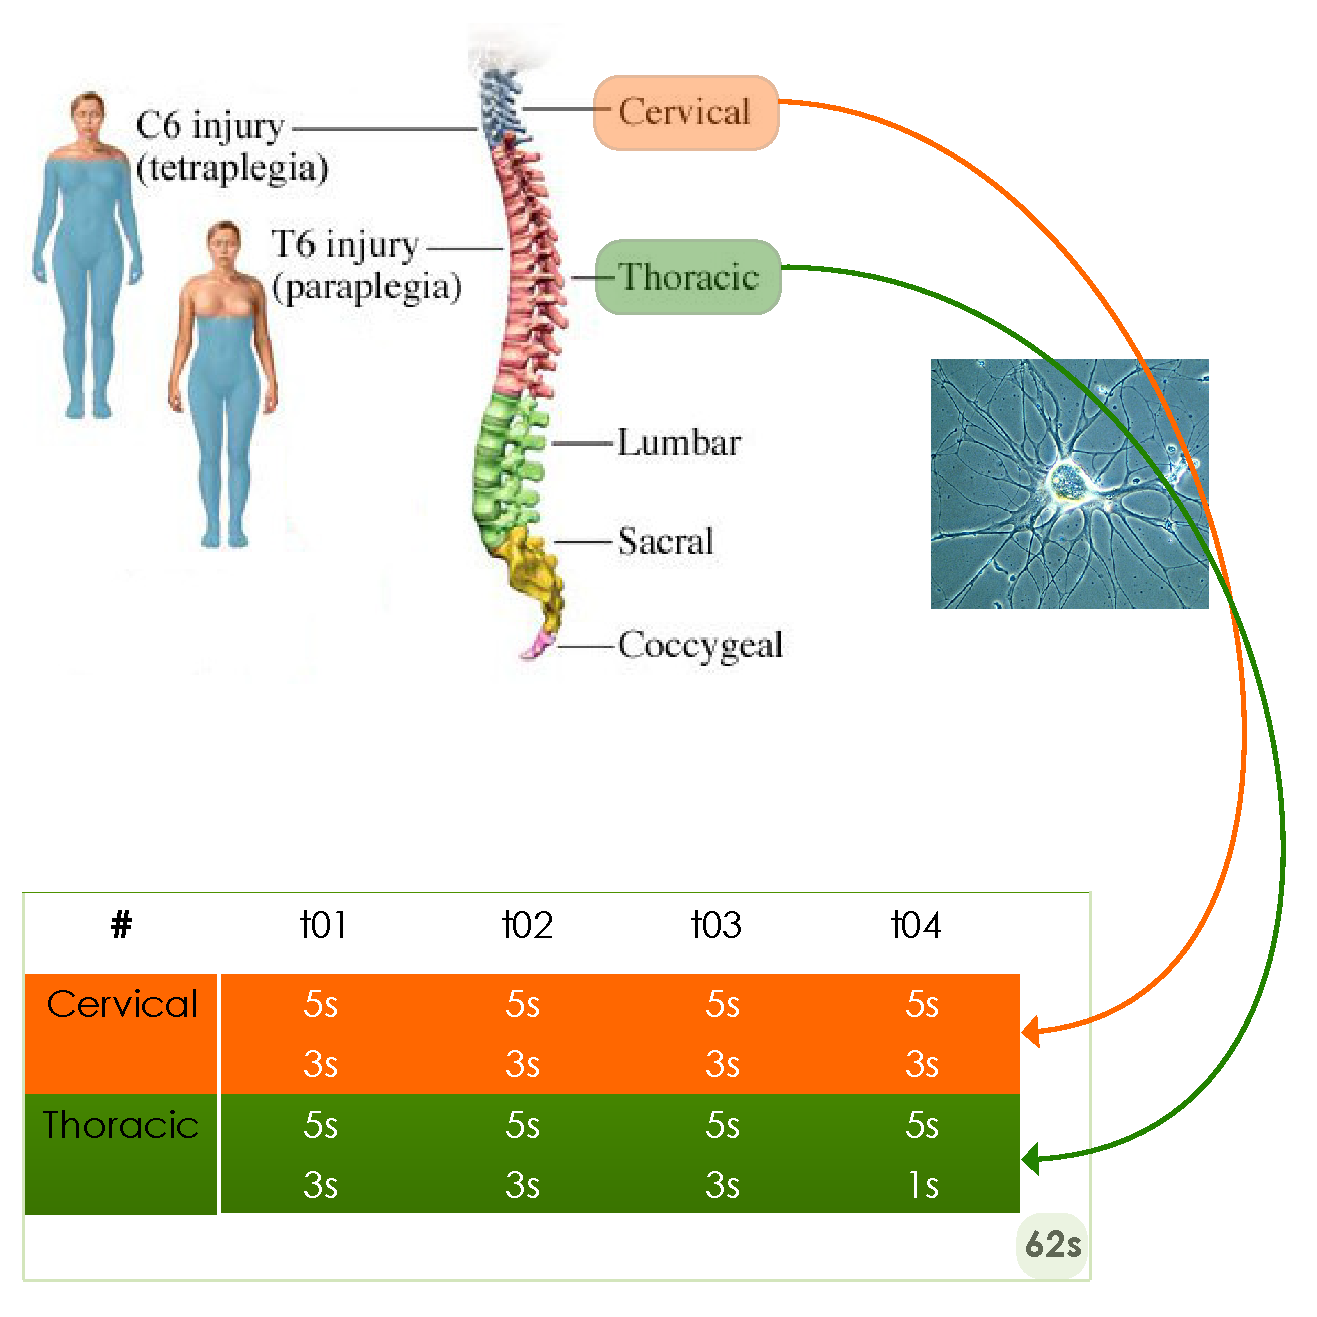
\includegraphics[width=\textwidth,height=\textheight,keepaspectratio]{img/descan2/dataset.png}
\caption[DEScan2 dataset illustration]{An illustration of our extraction of the \cite{Su2017} dataset.}
\label{fig:atacdataset}
\centering
\end{figure}

We downloaded the data from the \textit{GEO} database \cite{Edgar2002, Barrett2013} with accession number GSE82015\footnote{\url{https://www.ncbi.nlm.nih.gov/geo/query/acc.cgi?acc=GSE82015}} and mapped raw data using \textit{STAR} \cite{Dobin2013} with default parameter on Mus Musculus Genome ver.10 (mm10).

In order to detect the open chromatin regions we run our peak caller, cutting the genome in bins of 50bp and using running windows of minimum 50bp and maximum 1000bp. In such a way we are able to detect not just broad peak, but also smaller peaks.

To be confident with our results we compared the DEScan2 detected peaks on two genes (Arc and Gabrr1) with the same genes validated in \cite{Su2017}.
Lower part of figure \ref{fig:peaksdescan} shows the detected and validated regions (in blue and red) resulting differentially enriched between the E0 (in pink) and E1 (in green) samples, while the upper part shows DEScan2 peaks (in blue), which is able to catch the same regions of the published ones, but also (gold circles) to be more careful in the detection of smaller peaks.

\begin{figure}[H]
\includegraphics[width=\textwidth,height=\textheight,keepaspectratio]{img/descan2/peaks.png}
\caption[DEScan2 peaks detection]{A comparison of DEScan2 detected peaks with validated peaks in article \cite{Su2017}.}
\label{fig:peaksdescan}
\centering
\end{figure}

While it is very important to detect good peaks with a peak caller, it seems to be more relevant to detect reliable regions. Indeed, during the filtering step, the number of peaks depends not only by the peak score, but also by the number of replicates designed in the experiment.
The figure \ref{fig:filteringdescan} puts in relation these two relevant information. 
On the x-axis is represented the number of replicates, while on the y-axis the number of peaks is traced, and each line represents a different threshold for the score of the peaks, showing that higher is the threshold on the scores and the number of the replicates, lower is the number of the detected peaks.
Highlighting a proportional inversion between the number of the peaks and the number of the samples combined with the score of the detected regions.


\begin{figure}[H]
\includegraphics[width=\textwidth, height=\textheight, keepaspectratio]{img/descan2/filtering.png}
\caption[DEScan2 filtering step]{Filtering the detected regions with different thresholds on peak scores.}
\label{fig:filteringdescan}
\centering
\end{figure}


\begin{figure}[H]
\centering
\includegraphics[keepaspectratio]{img/descan2/counts.png}
\caption[DEScan2 counts illustration]{An illustration of the counts data structure produced by DEScan2.}
\label{fig:countsdescan}
\centering
\end{figure}










\subsection{Conclusions and Future Works} \label{sec:ticorseconclusions}
future: 
- load an existing project


%%%%%%%%%%%%%%%%%%%%%%%%%%%%%%
\chapter{Differential Enriched Scan 2\newline DEScan2} \label{sec:descan2cap}

Epigenetic, as shown in introduction (cite), is a pretty wide and complex field, and the sequencing technology to adopt depends on the biological question under investigation.

Some studies \cite{Koberstein2018, Auerbach2009} demonstrated the importance of genomewide chromatin accessibility of a broad spectrum of chromatin phenomena activation using sequencing techniques as \textit{Atac-Seq}, \textit{Sono-Seq}, etc.
Even if there are some methods for the analysis of these omic data types, there still is a lack of them, in particular for an emerging omic as \textit{Atac-Seq}.

To address this lack, we decided to create a useful instrument for analysing chromatine regions accessibility data (such as \textit{Atac-Seq}, \textit{Sono-Seq}).
Very often the biological questions to be answered, as for the RNA-Seq, need the comparison of two or more different biological conditions.
Starting from a set of already published \cite{Koberstein2018} scripts, we designed \gls{descan}, a software for helping the analysis of chromatin accession sequencing data.

\section{Introduction} \label{sec:descan2intro}
The \gls{descan} is an R \cite{Ihaka1996} tool developed for detecting open chromatin regions signal in order to facilitate the differential enrichment of genomic regions between two or more biological conditions.

The package has been implemented using Bioconductor \cite{Gentleman2004} data structures and methods, and it is available through Bioconductor repository since version 3.7.

The tool is organized in three main steps. 
A peak caller, which is a standard moving scan window that compares the reads coverage signal within a sliding window, to the signal in a larger region outside the window. It uses a Maximum Likelihood Estimator on a Poisson Distribution, providing a final score for each detected peak.

The filtering and alignment steps are aimed to determine if a peak is a "true peak" on the basis of its replicability in other samples. 
These steps are grouped in a single procedure and are based on a double user-defined threshold, one on the peaks's scores and one on the number of samples.

The third step produces a counts matrix where each column represents a sample and each row a peak. The value of each cell represents the number of reads for the peak in the sample.

The so produced counts matrix, as illustrated in the figure \ref{fig:descan2flow}, is useful both for doing differential enrichment between multiple conditions and for integrating the epigenomic data with other -omic data types.





\section{Methods} \label{sec:descan2methods}
\subsection{The interface}
\gls{igro} is a web platform fully developed in R with aid of Shiny libraries, combining the power of the R statistical instrument with HTML5/javascript flexibility.

Shiny apps are tipically designed for small applications, allowing a very easy and versatile way for developing and releasing them.
The basic structure of a shiny app is based on two main entities, the \gls{sui} and the \gls{ss}.
The first one includes all the aesthetic components which the user interact with, while the \gls{ss} processes all the computations.

Natively, shiny apps supports only one server, but when the needs grow up and multiple interfaces are needed the things become more complicated. 

Our case is composed of high number of methodologies for multiple-omics problem solving and required a more complex implementation.
To account our problematic, we choose to build \gls{igro} as self containing modules, by using recently born shiny modules technology \footnote{\url{https://shiny.rstudio.com/articles/modules.html}}.
In such a way, the main shiny app can be shredded in multiple "mini apps", each one with its own \gls{sui} and \gls{ss}.
This approach is totally invisible to the final user, but helps the developer for the maintainability and the extensibility of the entire tool.
Indeed, when future needs arise for the implementation of novel functionalities, it is necessary just to implement a novel module.

Our tool presents itself with an upper menu of main topics organized by main scopes. 
For each of these topics, a sub-menu with specific functionalities is available.
When additional functionalities are available, they appears in a left side menu.
In order to well setup the parameters for each functionality, an additional side menu is presented with the parameters and their possible values for the right setup (figure \ref{fig:integrhomain} shows a general representation of the main interface).

\begin{figure}[H]
\centering
\includegraphics[width=\textwidth, keepaspectratio]{img/integrho/interface.png}
\caption[\gls{igro} main interface]{\gls{igro} main interface description. A main menu in the upper part is presented with all the available main functionalities, and a left side menu is presented with additional functionalities (in blue). Red part indicates the settings for each functionality within the parameter setup. While in green results in table or graphical form are presented.}
\label{fig:integrhomain}
\end{figure}

Once the user set up the required parameters and used the section button the results are shown in graphical or table format in the main part of the interface.

Before to proceed to data analysis, it is mandatory for the user to setup the project with a dedicated interface. 
The user has to upload a design file which describes the information related to its samples, some of them are mandatory as the filename (with path) of the BAM files and the condition of each sample, while others are optional as the tissue or the run id. 
It is also possible to manually edit the design matrix directly from the interface (figure \ref{fig:integrhodesign}).

\begin{figure}[H]
\centering
\includegraphics[width=\textwidth, keepaspectratio]{img/integrho/design.png}
\caption[integrho design interface]{A screenshot of the project design \gls{igro} interface.}
\label{fig:integrhodesign}
\end{figure}

Using the project interface, \gls{igro} creates inside the working directory (returned by the \lstinline!getwd()! function) a dedicated folder with all the required subfolders and stores all the basic information of the project into an ad-hoc designed \lstinline!R6ProjectClass!, which is re-used during the whole session to speed up the configuration of each step of the analysis.


\subsection{Available Methodologies}

Unlike tools as Galaxy \cite{Hillman-Jackson2012} and Taverna \cite{Wolstencroft2013}, focused on analysis workflows, \gls{igro} gives to the user high freedom of interaction, reporting all performed steps in a human readable \textit{HTML} report.
 
It implements not only the methodologies reported inside \textit{ticorser} for \textit{RNA-Seq} and \textit{DEScan2} for \textit{ATAC-Seq}, but implements also methodologies for \textit{ChIP-Seq} data analysis, complementing these aspects by providing functionalities for their integration at different levels, such as functional enrichment with Gene Ontology and Pathways and peaks-genes annotation.

\begin{figure}[H]
\centering
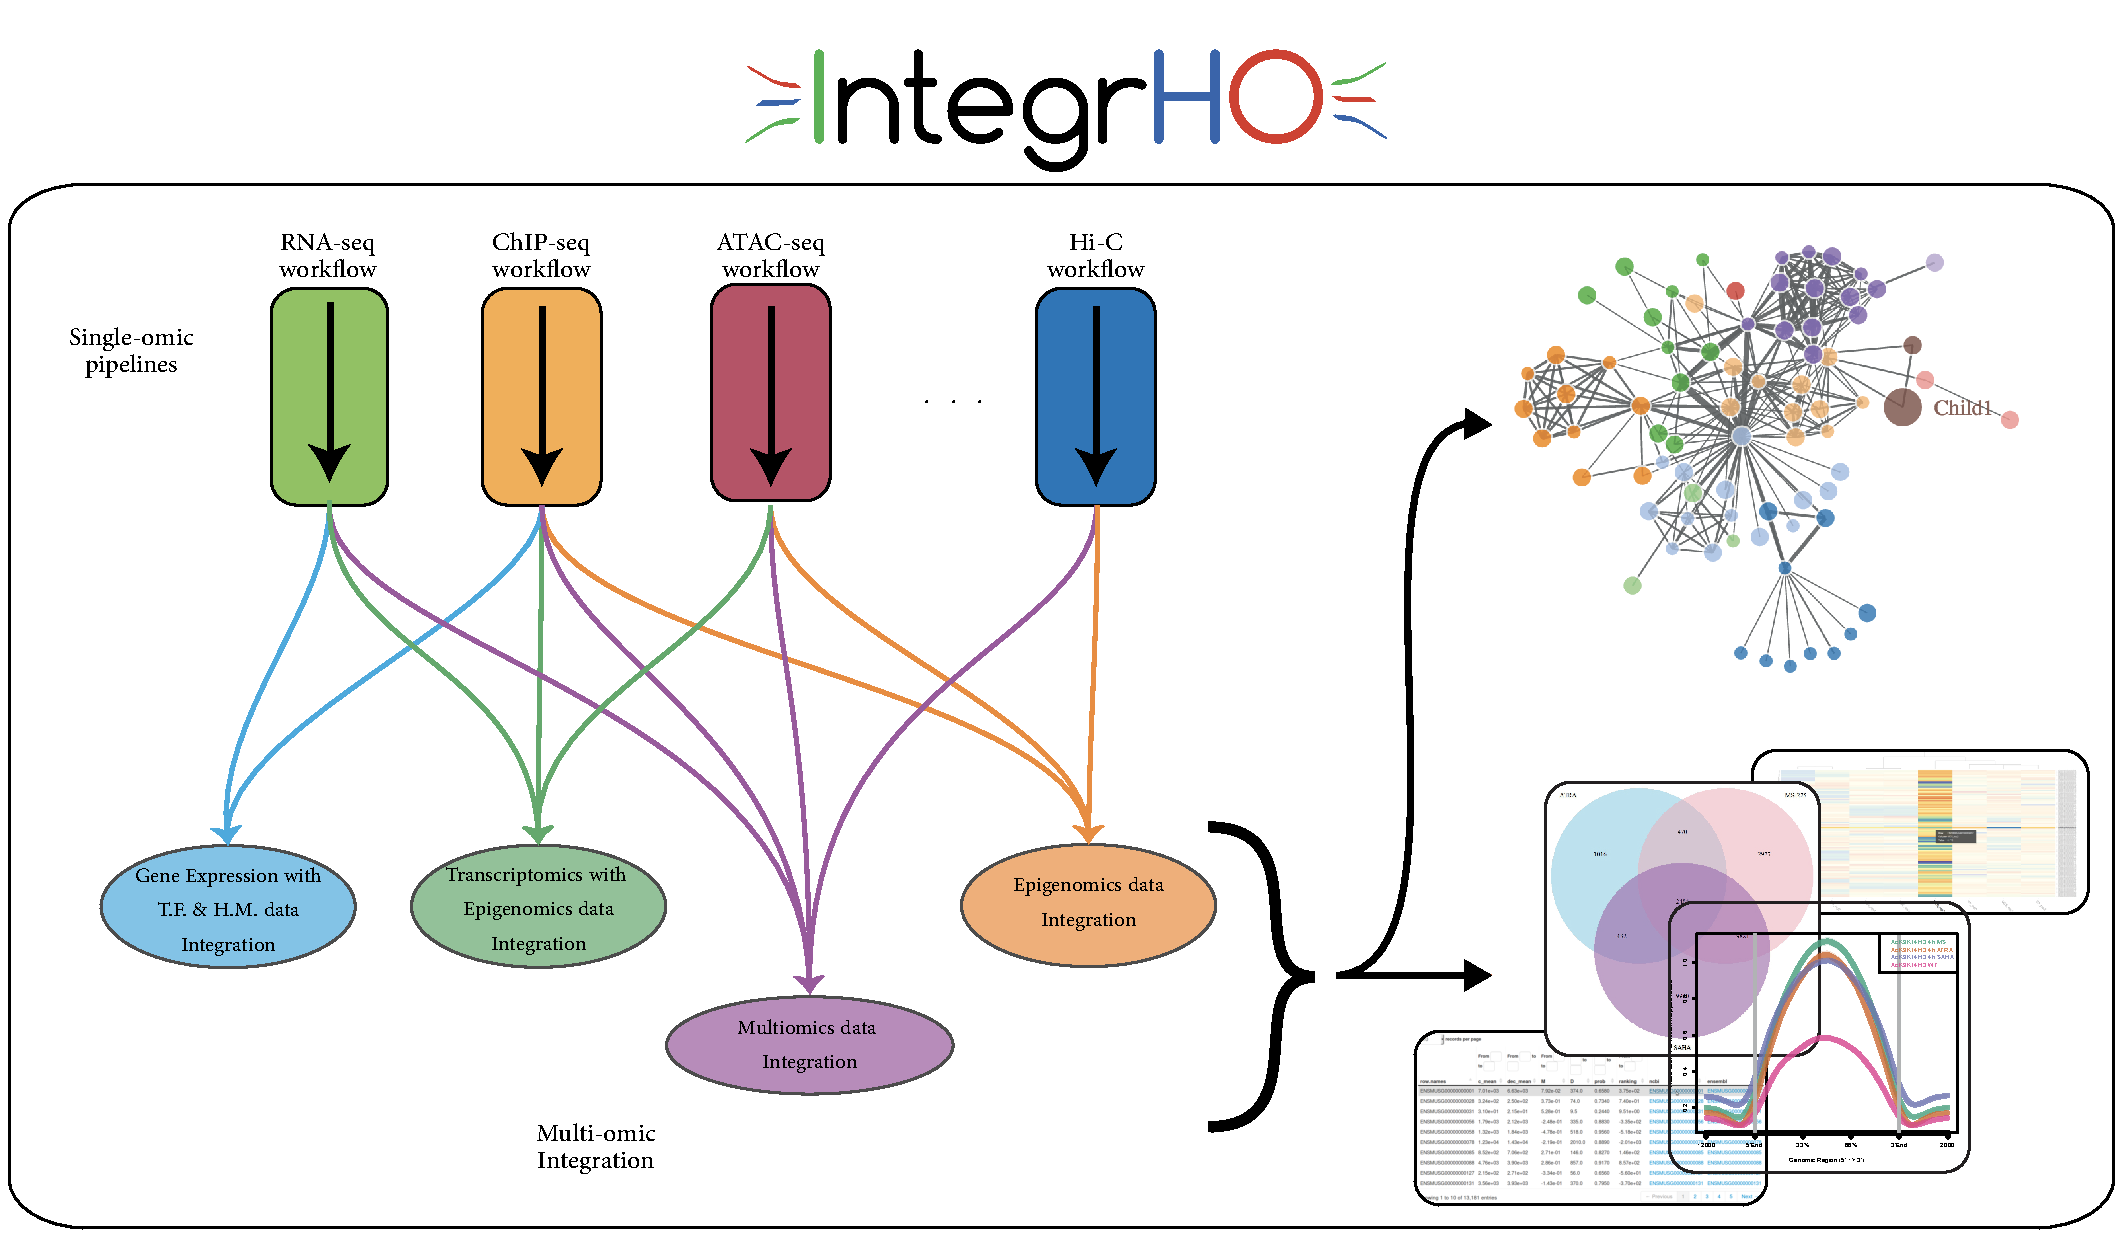
\includegraphics[width=\textwidth, keepaspectratio]{img/integrho/integrho_scheme.pdf}
\caption[integrho representation]{A schematical representation of \gls{igro} underlying idea.}
\label{fig:integrhoidea}
\end{figure}

For each -omics, \gls{igro} takes as input BAM or BED files, previously defined inside the design matrix of the main project definition interface.

Moreover, not only our software offers lots of utilities for data management and analysis, but also a great variability of graphics, useful to explore data and results, both in pre-processing and post-processing phase, such as \textit{barplots}, \textit{correlation plots}, \textit{heatmap}, \textit{scatterplots}, etc.

In order to facilitate the multi-omic data integration, we assembled several R functions to be freely combined in order to analyse each single-omic data type and to use their results for multi-omic data integration (Figure 1).

For \textit{RNA-seq} we constructed a dedicated interface for each step of a standard \textit{RNA-seq} data analysis pipeline, such as to build a count matrix, to filter out low counts with multiple tests, to normalize them and to account for batch effect.
Moreover, we selected multiple methods for \gls{deg}, such as \textit{edgeR}, \textit{DESeq2}, \textit{NOISeq}.

For \textit{ChIP-Seq} we constructed specific interfaces for peak calling, annotation and \glspl{der} detection.
For the peak calling, because of the lack of specific methods starting from BAM files, we implemented a dedicated interface for \textit{csaw}\cite{Lun2015} peak caller, which allows quantification for both broad and narrow peaks, typically resulting from \gls{hm} and \gls{tf} \textit{ChIP-seq} data.

For the annotation we selected the \textit{ChIPpeakAnno} and the \textit{ChIPseeker} R/Bioconductor packages, which produces similar output formats starting from peaks.
While for the detection of \glspl{der} we used the same methods as for \textit{RNA-seq}.

For \textit{ATAC-Seq} we used mostly the same methods implemented for the \textit{ChIP-Seq}, but designing specific interfaces for the filtering/alignment and the counting matrix as implemented in the \textit{DEScan2} package (see chapter \ref{sec:descan2cap} for further details).

To provide an integration of these -omics, we dedicated an entire section to this aspect, with functionalities for the annotation of \glspl{der} with \glspl{deg} using \textit{ChIPpeakAnno} and to use this information to investigate the functional response by enrichment for Gene Ontology or for Pathways.
These last two aspects implemented with aid of \textit{g:Profiler} \cite{Reimand2016} and \textit{graphite} \cite{Sales2012a} R/Bioconductor packages.


\subsection{Peak Caller} \label{sec:descan2peakcall}
The Peak Caller (defined by the \lstinline!findPeaks! function) takes as input a set of alignment files (BAM \cite{Li2009} or BED format) with the code identifier for the reference genome (i.e. \textit{mm10} for Mus Musculus version 10) and several additional parameters, useful for the peak detection setup.

The alignment data are stored as an object of class \textit{GenomicRangesList} \cite{Lawrence2013}, where each element represents a file. 
In order to facilitate the parallelization of the computations over the chromosomes, the list is re-arranged as a chromosome list of \textit{GenomicRangesList}, where each element represents the file containing just the \textit{GenomicRanges} of the specific chromosome (see section \ref{sec:descan2addfeat} for a detailed description of this procedure).

For each element of this data structure, the algorithm firstly divides each chromosome into bins of \lstinline!binSize! parameter length (the default value is 50bp) and then computes the reads coverage of the bins with moving scan windows, spanning from \lstinline!minWin! to \lstinline!maxWin! parameters of \lstinline!binSize! interval.

In order to be able to catch narrow and broad peaks, the algorithm computes the coverage also using windows of two different lengths, that can be defined with \lstinline!minCompWinWidth! and \lstinline!maxCompWinWidth! (defaults values are 5000bp and 10000bp) parameters, computing a matrix of $n$ bins and $p$ windows.
%\textit{\textbf{for real this part is to construct a sort of background of the signal, to compare the smaller windows to - ask to davide?}}

The coverage matrix is useful to merge contiguous regions and to compute a score for each of them, applying a \gls{mle}, assuming a \textit{Poisson} distribution of the coverage across the windows.

Formalizing: assuming that each window is distributed as a \textit{Poisson} random variable, we assume to observe the $n$ coverages as an IID sequence $X_n$. Thus, the probability mass function is described as:

\[ p(x_i) = \frac{\lambda^{x_i}}{{x_i!}} exp(-\lambda) \]

Where the integer nature of the data support the Poisson distribution as the set of non-negative integer number and where $\lambda$ is the Poisson parameter to estimate with a \gls{mle}, described as the estimator:

\[\hat{\lambda}_n=\frac{1}{n}\sum_{i=1}^{n}x_i\]

Which corresponds to the sample mean of the \textit{n} observations in the sample.

In order to define a score for the peaks, we defined a z-score for each bin-window as follow:

\[ \hat{z}_n=\frac{x_n - \hat{\lambda} }{\sqrt{\hat{\lambda}}} \]

Subsequently, an iterative algorithm detects the maximum z-score, between all the windows, at each step, and then detects all the contigs bins with a not 0 value, across all the windows.
In such a way a peak is defined by the starting base of the ''lowest'' bin to the last base of the ''highest'' contigous bin, assigning the maximum z-score between all the detected contigs bins.

Additionally, on user request, the function provides as output, for each alignment file, a \gls{tsv} file within the regions coordinates and the score of the detected peaks.




\subsection{Peak Filtering and Alignment} \label{sec:descan2filtering}


Basing on this idea, the filtering step is developed to filter out those peaks not present in at least a user-defined number of samples. In the light of this, the user can decide the min-
imum number of samples where each peak has to be detected. A further threshold can be used over
the peak score.

\subsection{Counting Peaks} \label{sec:descan2peakcounts}
The counting step (\lstinline{countFinalRegions} method) is designed to take a \textit{GenomicRanges} data structure as input, where for each peak additional attributes, as the score and the number of samples, are saved.
Moreover, to quantify the peaks given as input, it requires also the path of the BAM/BED files where the reads are stored.

For each region the method counts the number of reads present in each sample.
In so doing, it produces as result a matrix of the counts, where the rows and the columns, respectively, represent the regions and the samples.

In order to keep trace of all information associated to the regions, it produces a \textit{SummarizedExperiment} \cite{SummExp} data structure, giving the possibility to retrieve the \textit{GenomicRanges} of associated peaks and the count matrix, respectively, using \lstinline{rowRanges} and \lstinline{assays} method.

The choice to produce a count matrix is guided by the versatility of this data structure, useful not only for the differential enrichment of the regions between multiple conditions, but also for integrating the epigenomic data with other -omics, as RNA-Seq.

\subsection{Additional Features} \label{sec:descan2addfeat}
\gls{tic} offers multiple additional features to help the user during the differential enrichment analysis of time-course \textit{RNA-seq} data.

\subsubsection{Gene quantification}

A fundamental aspect during \textit{RNA-seq} analysis is the quantification of the features (genes).
To account for this, \gls{tic} give the possibility to quantify the gene expression, starting from samples mapping files, using the \lstinline!countBamFilesFeatureCounts! function with the aim to guide and facilitate this operation to the user.

The feature is based on the \lstinline!featureCounts! method available through the \textit{Rsubread} R/Bioconductor package \cite{Liao2013}, hard coding some parameters as \lstinline!useMetafeatures! to \lstinline!TRUE! and \lstinline!allowMultiOverlap! to \lstinline!FALSE!.
The user can give as input a list of \textit{BAM} files and a \gls{gtf} file, choosing  the \lstinline!gtf.attr.type! and \lstinline!gtf.feat.type! to quantify the samples expression on its needs.

\subsubsection{Results Comparison}

Usually during a differential expression analysis it is pretty common to have the need to compare multiple \glspl{deg} results list.
In order to facilitate this need we developed three different functions for \textit{Venn} diagrams, \lstinline!Venn2de!, \lstinline!Venn3de! and \lstinline!Venn4de!, respectively for two, three and four lists.
During this process it is often required not just to show the graphical plot, but it's most important to show the gene lists resulting from the intersections and disjunctions of the Venns.
To afford this aim these functions take as input the gene lists to compare and automatically store output file lists within the resulting lists of all the areas of the produced Venns.

\subsubsection{Gene Identifiers Conversion}

The \gls{tic} package exports multiple functions for the gene names manipulation. 
Indeed, it is very common the need to convert \glspl{deg} list from a specific identifier to another.
We developed \lstinline!convertGenesViaMouseDb! and \lstinline!convertGenesViaBiomart! which convert a \glspl{deg} list using the \textit{org.Mm.eg.db} \cite{Carlson2018} for \textit{Mouse} and using the \textit{biomaRt} R/Bioconductor package for \textit{Human, Mouse} and \textit{Rat}.
Additionally, it's possible to easily attach the resulting list to a \textit{dataframe}, by using the \lstinline!attachGeneColumnToDf! function, which takes care of adding a new column within the mapped identifiers in the right places of the original \textit{dataframe}.

\subsubsection{Input/Output File Handling}

To speed up the reading and writing of input/output files, \gls{tic} offers two main functions, \lstinline!readDataFrameFromTSV! and \lstinline!writeDataFrameAsTSV!.

In the first case there is only one mandatory parameter, the \lstinline!file.name.path!, even if gives the possibility to change the classical parameters as \lstinline!row.names.col, headed.flag, sep, quote.char!.

While in the second case the function requires the \lstinline!data.frame.to.save! and the \lstinline!file.name.path! where to store the object. 
Also in this case it is possible to set the classical parameters as \lstinline!col.names! and \lstinline!row.names!.

Moreover, we implemented a method for creating a folder path in a recursive way.
The \lstinline!updateFolderPath! method takes as input a starting path and a list of strings. 
It is useful when using a recursive function call or an automated nested function call process.
Of course if a user need to create a single path by itself, he/she can simply create it using the \lstinline!dir.create! R base function.




















\section{Case Study} \label{sec:descan2results}
\textbf{A few words on epigenomic data}

We illustrate the performances of DEScan2 using a dataset \cite{Su2017} describing adult mouse dentate granule neurons in vivo before and after synchronous neuronal activation using Atac-Seq and RNA-Seq technologies (see sections \ref{sec:atacseq} and \ref{sec:rnaseq}).

This dataset is organized in 62 samples of Atac-Seq and RNA-Seq, sampling them at different time points, with four replicates for time point.
Of this samples we chose to compare the differences at the first two stages, time 0 (E0) and After 1 hour of neuronal induction (E1), in order to show a possible Atac-Sec workflow for Differential Enrichment, and how to integrate this type of data with RNA-Seq data.

\begin{figure}[H]
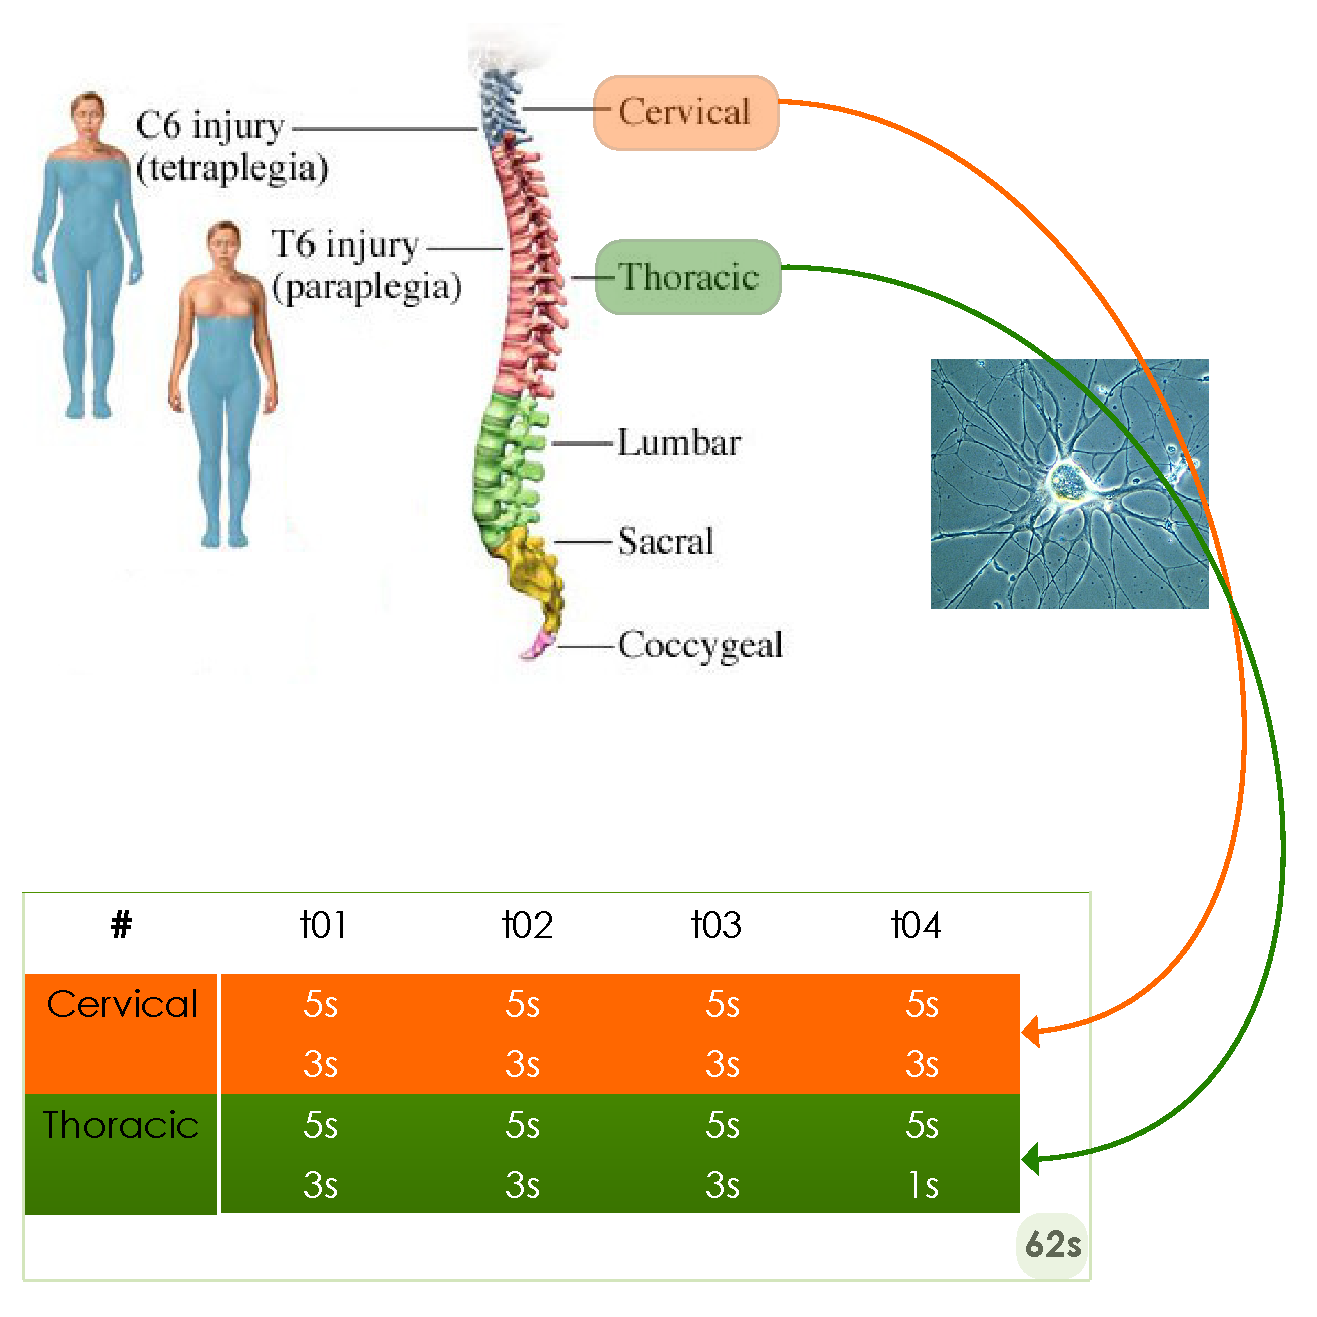
\includegraphics[width=\textwidth,height=\textheight,keepaspectratio]{img/descan2/dataset.png}
\caption[DEScan2 dataset illustration]{An illustration of our extraction of the \cite{Su2017} dataset.}
\label{fig:atacdataset}
\centering
\end{figure}

We downloaded the data from the \textit{GEO} database \cite{Edgar2002, Barrett2013} with accession number GSE82015\footnote{\url{https://www.ncbi.nlm.nih.gov/geo/query/acc.cgi?acc=GSE82015}} and mapped raw data using \textit{STAR} \cite{Dobin2013} with default parameter on Mus Musculus Genome ver.10 (mm10).

In order to detect the open chromatin regions we run our peak caller, cutting the genome in bins of 50bp and using running windows of minimum 50bp and maximum 1000bp. In such a way we are able to detect not just broad peak, but also smaller peaks.

To be confident with our results we compared the DEScan2 detected peaks on two genes (Arc and Gabrr1) with the same genes validated in \cite{Su2017}.
Lower part of figure \ref{fig:peaksdescan} shows the detected and validated regions (in blue and red) resulting differentially enriched between the E0 (in pink) and E1 (in green) samples, while the upper part shows DEScan2 peaks (in blue), which is able to catch the same regions of the published ones, but also (gold circles) to be more careful in the detection of smaller peaks.

\begin{figure}[H]
\includegraphics[width=\textwidth,height=\textheight,keepaspectratio]{img/descan2/peaks.png}
\caption[DEScan2 peaks detection]{A comparison of DEScan2 detected peaks with validated peaks in article \cite{Su2017}.}
\label{fig:peaksdescan}
\centering
\end{figure}

While it is very important to detect good peaks with a peak caller, it seems to be more relevant to detect reliable regions. Indeed, during the filtering step, the number of peaks depends not only by the peak score, but also by the number of replicates designed in the experiment.
The figure \ref{fig:filteringdescan} puts in relation these two relevant information. 
On the x-axis is represented the number of replicates, while on the y-axis the number of peaks is traced, and each line represents a different threshold for the score of the peaks, showing that higher is the threshold on the scores and the number of the replicates, lower is the number of the detected peaks.
Highlighting a proportional inversion between the number of the peaks and the number of the samples combined with the score of the detected regions.


\begin{figure}[H]
\includegraphics[width=\textwidth, height=\textheight, keepaspectratio]{img/descan2/filtering.png}
\caption[DEScan2 filtering step]{Filtering the detected regions with different thresholds on peak scores.}
\label{fig:filteringdescan}
\centering
\end{figure}


\begin{figure}[H]
\centering
\includegraphics[keepaspectratio]{img/descan2/counts.png}
\caption[DEScan2 counts illustration]{An illustration of the counts data structure produced by DEScan2.}
\label{fig:countsdescan}
\centering
\end{figure}










\section{Conclusions and Future Works} \label{sec:descan2next}
future: 
- load an existing project


%%%%%%%%%%%%%%%%%%%%%%%%%%%%%%%%%%%%%%%%%%
\chapter{IntegrHO - Integration of High-Throughtput Omics data}
\section{Introduction}
\section{Methods}
\subsection{Single Omic Approach}
\subsection{Multi Omic Approach}
\subsubsection{Low Level Itegration}
\subsubsection{High Level Itegration}
\section{Implementation Aspects}
\section{Reproducible Computational Research}
\section{Results}
\chapter{Conclusions \& Future Works}
%%%%%%%%%%%%%%%%%%%%%%%%%%%%%%%%%%%%%%

\chapter{Reproducible Computational Research}

\begin{appendices}
\section{R Language}
\section{R Markdown Language}
%\include{appendixA}
%\include{appendixB}
%\include{appendixC}
\end{appendices}

%This chapter explains some basic information useful to understand the context where this thesis work has been developed.
Explaining some biological basic aspects and how it is possible to study the cellular behaviour from multiple points of view using different sequencing techniques.
%\include{aim_of_the_study}
%\include{MVDA}
%\include{INSIdEnano}
%\include{discussion}
%\include{conclusion}

%\begin{appendices}
%\include{appendixA}
%\include{appendixB}
%\include{appendixC}
%\end{appendices}
%\makeglossaries


\printbibliography[heading=bibnumbered]
\cleardoublepage

\printglossaries

\cleardoublepage
% \phantomsection
\addcontentsline{toc}{chapter}{\listfigurename}
\listoffigures

\cleardoublepage
% \phantomsection
\addcontentsline{toc}{chapter}{\listtablename}
\listoftables

%\listoffigures
%\listoftables

\end{document}